\documentclass[tikz]{standalone}
\usepackage{pgfplots}
\usepgfplotslibrary{statistics}
\def\axisdefaultwidth{6cm}
\def\axisdefaultheight{6cm}
\usetikzlibrary{pgfplots.colorbrewer}
\begin{document}
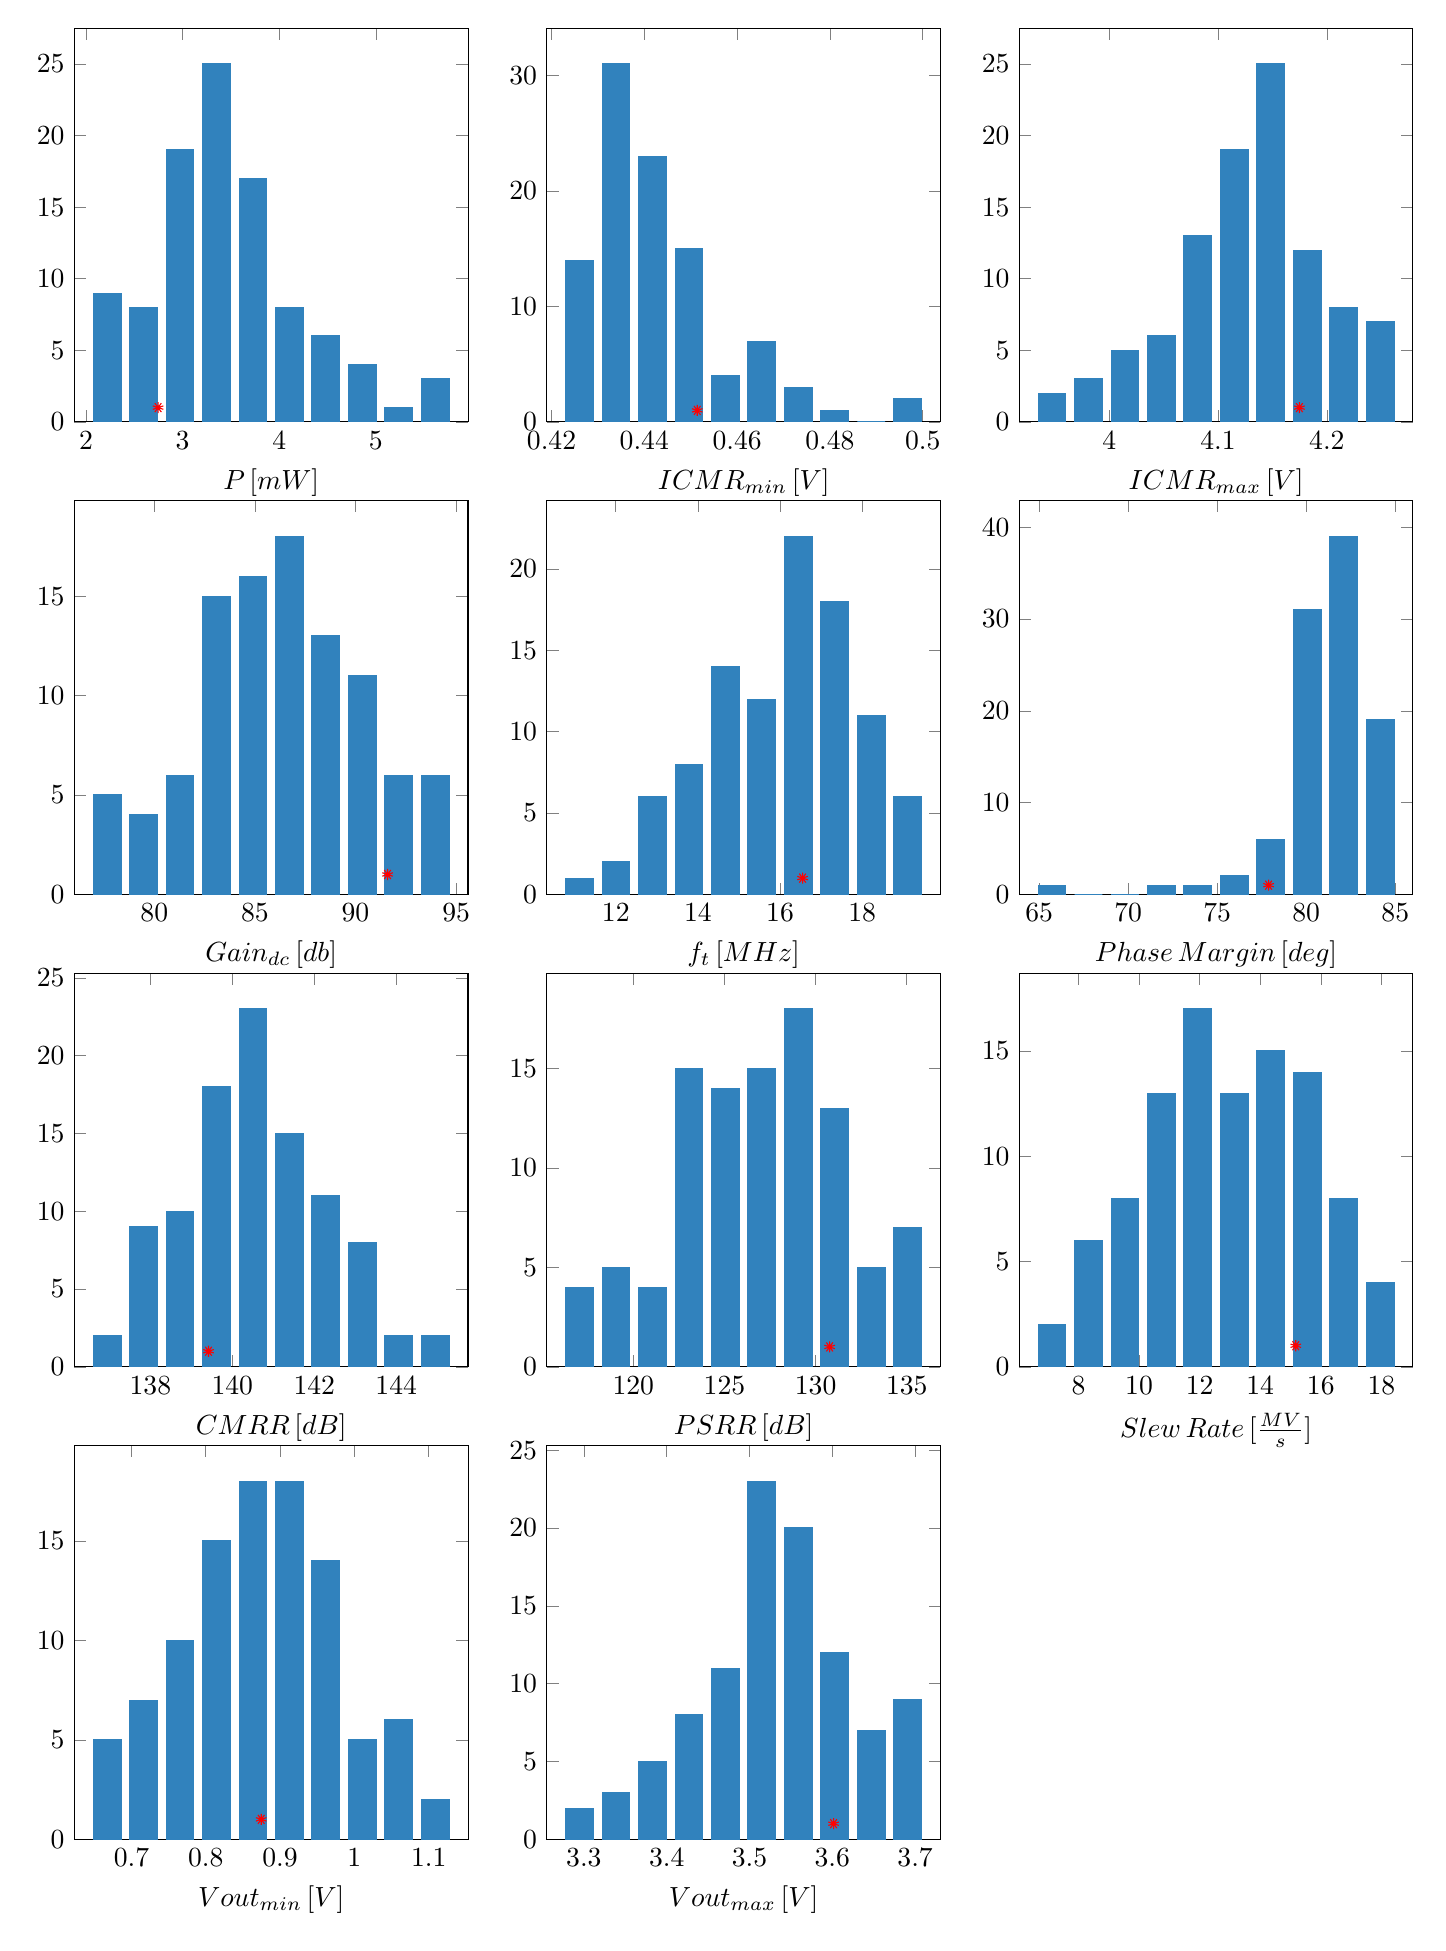
\begin{tikzpicture}
\begin{axis}[scale only axis, width=5cm, height=5cm, at={(0cm,0cm)},ymin=0, xlabel={$P \, [mW]$}]
\addplot [
ybar,
fill=Blues-I,
draw=Blues-I]
table [x=perf, y=cnt] {
cnt                 perf                
9                   2.219585            
8                   2.5967915           
19                  2.9739980000000004  
25                  3.3512045           
17                  3.728411            
8                   4.1056175           
6                   4.482824            
4                   4.860030500000001   
1                   5.237237            
3                   5.6144435           
};
\addplot[mark=10-pointed star, red] coordinates {(2.74644,1)};
\end{axis}
\begin{axis}[scale only axis, width=5cm, height=5cm, at={(6cm,0cm)},ymin=0, xlabel={$ICMR_{min} \, [V]$}]
\addplot [
ybar,
fill=Blues-I,
draw=Blues-I]
table [x=perf, y=cnt] {
cnt                 perf                
14                  0.4260514           
31                  0.43390789          
23                  0.44176438          
15                  0.44962087          
4                   0.45747736          
7                   0.46533385000000005 
3                   0.47319034000000004 
1                   0.48104683000000004 
0                   0.48890332000000003 
2                   0.49675981          
};
\addplot[mark=10-pointed star, red] coordinates {(0.4514005,1)};
\end{axis}
\begin{axis}[scale only axis, width=5cm, height=5cm, at={(12cm,0cm)},ymin=0, xlabel={$ICMR_{max} \, [V]$}]
\addplot [
ybar,
fill=Blues-I,
draw=Blues-I]
table [x=perf, y=cnt] {
cnt                 perf                
2                   3.947446            
3                   3.9809428           
5                   4.0144396           
6                   4.0479364           
13                  4.0814332           
19                  4.11493             
25                  4.1484268           
12                  4.1819236           
8                   4.2154204           
7                   4.2489172           
};
\addplot[mark=10-pointed star, red] coordinates {(4.17473,1)};
\end{axis}
\begin{axis}[scale only axis, width=5cm, height=5cm, at={(0cm,-6cm)},ymin=0, xlabel={$Gain_{dc} \, [db]$}]
\addplot [
ybar,
fill=Blues-I,
draw=Blues-I]
table [x=perf, y=cnt] {
cnt                 perf                
5                   77.65856            
4                   79.470236           
6                   81.28191199999999   
15                  83.093588           
16                  84.90526399999999   
18                  86.71694            
13                  88.528616           
11                  90.34029199999999   
6                   92.151968           
6                   93.96364399999999   
};
\addplot[mark=10-pointed star, red] coordinates {(91.59476,1)};
\end{axis}
\begin{axis}[scale only axis, width=5cm, height=5cm, at={(6cm,-6cm)},ymin=0, xlabel={$f_{t} \, [MHz]$}]
\addplot [
ybar,
fill=Blues-I,
draw=Blues-I]
table [x=perf, y=cnt] {
cnt                 perf                
1                   11.119491415415192  
2                   12.007003625743094  
6                   12.894515836071     
8                   13.782028046398903  
14                  14.669540256726807  
12                  15.557052467054708  
22                  16.444564677382612  
18                  17.332076887710517  
11                  18.21958909803842   
6                   19.107101308366325  
};
\addplot[mark=10-pointed star, red] coordinates {(16.547820400953846,1)};
\end{axis}
\begin{axis}[scale only axis, width=5cm, height=5cm, at={(12cm,-6cm)},ymin=0, xlabel={$Phase \, Margin \, [deg]$}]
\addplot [
ybar,
fill=Blues-I,
draw=Blues-I]
table [x=perf, y=cnt] {
cnt                 perf                
1                   65.72676738013709   
0                   67.77374029247137   
0                   69.82071320480564   
1                   71.86768611713993   
1                   73.91465902947421   
2                   75.96163194180849   
6                   78.00860485414276   
31                  80.05557776647704   
39                  82.10255067881133   
19                  84.1495235911456    
};
\addplot[mark=10-pointed star, red] coordinates {(77.8858766294097,1)};
\end{axis}
\begin{axis}[scale only axis, width=5cm, height=5cm, at={(0cm,-12cm)},ymin=0, xlabel={$CMRR \, [dB]$}]
\addplot [
ybar,
fill=Blues-I,
draw=Blues-I]
table [x=perf, y=cnt] {
cnt                 perf                
2                   136.94572           
9                   137.83527999999998  
10                  138.72484           
18                  139.6144            
23                  140.50396           
15                  141.39352           
11                  142.28307999999998  
8                   143.17264           
2                   144.0622            
2                   144.95176           
};
\addplot[mark=10-pointed star, red] coordinates {(139.41881,1)};
\end{axis}
\begin{axis}[scale only axis, width=5cm, height=5cm, at={(6cm,-12cm)},ymin=0, xlabel={$PSRR \, [dB]$}]
\addplot [
ybar,
fill=Blues-I,
draw=Blues-I]
table [x=perf, y=cnt] {
cnt                 perf                
4                   117.0563            
5                   119.055639          
4                   121.05497799999999  
15                  123.054317          
14                  125.05365599999999  
15                  127.052995          
18                  129.052334          
13                  131.051673          
5                   133.051012          
7                   135.050351          
};
\addplot[mark=10-pointed star, red] coordinates {(130.77000999999998,1)};
\end{axis}
\begin{axis}[scale only axis, width=5cm, height=5cm, at={(12cm,-12cm)},ymin=0, xlabel={$Slew \, Rate \, [\frac{MV}{s}]$}]
\addplot [
ybar,
fill=Blues-I,
draw=Blues-I]
table [x=perf, y=cnt] {
cnt                 perf                
2                   7.12833             
6                   8.331536999999999   
8                   9.534744            
13                  10.737950999999999  
17                  11.941158           
13                  13.144364999999999  
15                  14.347572           
14                  15.550778999999999  
8                   16.753985999999998  
4                   17.957193           
};
\addplot[mark=10-pointed star, red] coordinates {(15.1724,1)};
\end{axis}
\begin{axis}[scale only axis, width=5cm, height=5cm, at={(0cm,-18cm)},ymin=0, xlabel={$Vout_{min} \, [V]$}]
\addplot [
ybar,
fill=Blues-I,
draw=Blues-I]
table [x=perf, y=cnt] {
cnt                 perf                
5                   0.6672908           
7                   0.71634962          
10                  0.76540844          
15                  0.81446726          
18                  0.86352608          
18                  0.9125849           
14                  0.9616437200000001  
5                   1.01070254          
6                   1.05976136          
2                   1.1088201800000002  
};
\addplot[mark=10-pointed star, red] coordinates {(0.8745919,1)};
\end{axis}
\begin{axis}[scale only axis, width=5cm, height=5cm, at={(6cm,-18cm)},ymin=0, xlabel={$Vout_{max} \, [V]$}]
\addplot [
ybar,
fill=Blues-I,
draw=Blues-I]
table [x=perf, y=cnt] {
cnt                 perf                
2                   3.294801            
3                   3.338822            
5                   3.3828430000000003  
8                   3.426864            
11                  3.470885            
23                  3.514906            
20                  3.558927            
12                  3.602948            
7                   3.646969            
9                   3.69099             
};
\addplot[mark=10-pointed star, red] coordinates {(3.601503,1)};
\end{axis}
\end{tikzpicture}
\end{document}
